\section{Funktionsweise}
\label{funktion}

Dieser Abschnitt erklärt die Arbeitsweise der Inversionsmethode im Allgemeinen. Danach wird kurz das Prinzip 
der Hashtabelle wiederholt, um danach die Funktionsweise der hash-basierten Inversionsmethode zu erläutern.


\subsection{Inversionsmethode}
Devroye \cite{devroye-non_uniform_random_variate-1986} beschreibt in seinem Buch die Inversionsmethode als eine 
Methode, bei der mithilfe des Inversen $F^{-1}$ einer bekannten Verteilungsfunktion $F$ und mit einer uniformen, 
zufälligen Zahl $U \in [0, 1]$ eine zufällige Zahl $X = F^{-1}(U)$ generiert wird. Dadurch gibt es eine monotone 
Beziehung zwischen $U$ und $X$, weshalb ein Paar $(x_1, x_2)$, bei dem $X_1$ und $X_2$ maximal anti-korreliert 
zueinander sind, mit 
\begin{equation}
    (F^{-1}(U),\, F^{-1}(1 - U))
\end{equation}
berechnet werden kann. Diese Eigenschaft wird vor allem in 
Simulationen benötigt.

Durch die Erzeugung der Zufallsvariable $X$ durch das Inverse einer Verteilungsfunktion kann die Inversionsmethode 
allerdings nur dann optimal angewandt werden, wenn $F^{-1}$ einfach zu berechnen ist oder sogar schon bekannt ist. 
Durch heutige numerische Algorithmen können aber auch Funktionen, welche nicht \glqq per Hand\grqq{} invertierbar sind, in der 
vorgestellten Weise benutzt werden. 

\begin{table}
    \centering
    \begin{tabular}{lll}
    Name         & Funktion & Zufällige Variable \\
                 &          &                    \\
    Exponentiell & $1 - e^{-x}$ & $\log(1/U)$ \\
    Logistisch   & $1 / (1 + e^{-x})$ & $-\log(\dfrac{1-U}{U})$ \\
    Cauchy       & $1/2 + (1/\pi) \arctan(x)$ & $\tan(\pi U)$
    \end{tabular}
    \caption{Explizit invertierbare Verteilungsfunktionen \cite{devroye-non_uniform_random_variate-1986}}
    \label{fig:invFuncs}
\end{table}

Nach Devroye können, nur unter Verwendung sogenannter \glqq einfachen Transformationen\grqq, Paare von unabhängigen 
Variablen generiert werden. Zum Beispiel kann mit der Standardnormalverteilung $\dfrac{e^{-x^2/2}}{\sqrt{2\pi}}$ ein Paar von 
unabhängigen, zufälligen standardnormalverteilten Variablen mit 
\begin{equation}
    (X, Y) = \bigg( \sqrt{\log(\dfrac{1}{U_1})}\cos(2\pi U_2),\, \sqrt{\log(\dfrac{1}{U_1})}\sin(2\pi U_2) \bigg)
    \label{eq:stdnormdensity}
\end{equation}
generiert werden. Dabei sind $U_1, U_2 \in [0, 1]$ unabhängige gleichverteile zufällige Variablen.

% \begin{figure}[!h]
%     \centering
%     \def\svgwidth{\columnwidth}
%     % inkscape -D image.svg  -o image.pdf --export-latex
%     \scalebox{1}{\input{../../Media/pdf_tex/examplePlot2.pdf_tex}}
%     \caption{(a) 500 Punkte mit einer logistischen Dichte auf der X- und Y-Achse (b) 500 Punkte standardnormalverteilt \eqref{eq:stdnormdensity}.}
%     \label{bild:examplePlot}
% \end{figure}
\begin{figure}
    \centering
    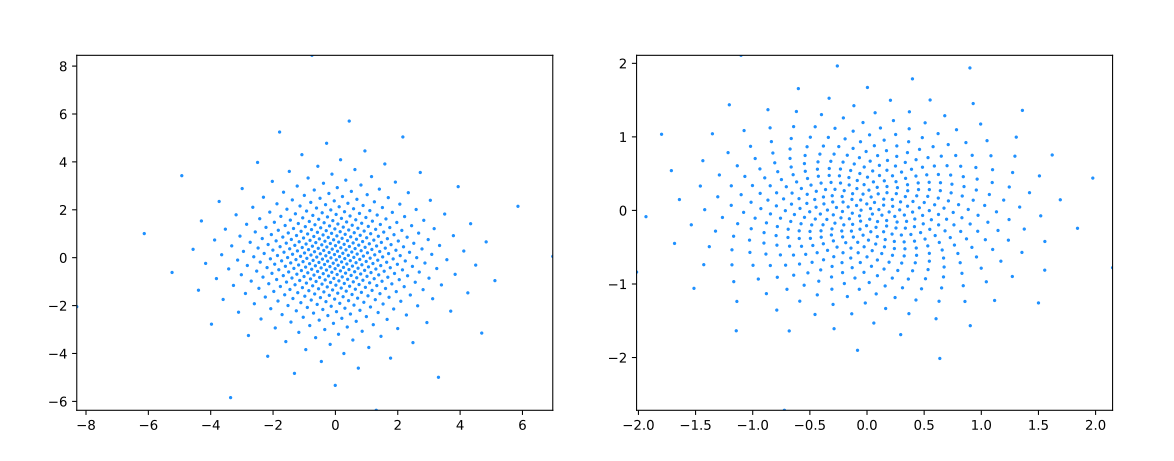
\includegraphics[width=0.48\textwidth]{fig1.png}
    \caption{(a) 500 Punkte mit einer logistischen Dichte auf der X- und Y-Achse (b) 500 Punkte standardnormalverteilt \eqref{eq:stdnormdensity}.}
    \label{bild:examplePlot}
\end{figure}


Bei einem Zufallsvektor $ (X_1, ..., X_n) \in \mathbb{R}^n$ wird die Inversionsmethode auf je eine Dimension angewandt 
und dann die folgende Zufallszahl generiert und dann rekursiv die nachfolgenden Dimensionen berechnet. Genauer bedeutet das, 
dass zuerst die Variable $X_n$ der höchsten Dimension berechnet wird. Danach wird $X_{n-1}$ mit der zugewiesenen Funktion 
berechnet, wobei $X_n$ als bedingte Verteilung mit eingerechnet wird.


\subsection{Hashtabelle}
Eine Hashtabelle ist eine Datenstruktur, die mithilfe einer Hashfunktion $H: V \rightarrow K$ einen Wert $v \in V$ 
auf den zugehörigen Schlüssel $k \in K$ ab. Die Werte werden dann in einem Array gespeichert, 
wobei der Schlüssel die Position angibt. Da es in der Praxis meistens mehr Werte als Stellen im Array gibt, treten 
allerdings Kollisionen auf. Diese können entweder dadurch gelöst werden, dass das Array pro Schlüssel eine verkettete 
Liste enthält. In diese werden dann die kollidierende Werte hintereinander geschrieben. Die zweite verbreitete Möglichkeit 
ist lineares Sondieren. Dabei wird der Wert immer an die nächste freie Stelle in der Hashtabelle, von seinem eigentlichem 
Platz aus gesehen, geschrieben.


\subsection{Inversion mit Hashing}
Um die Inversionsmethode zu beschleunigen, gibt es mehrere Möglichkeiten. Eine davon ist, 
eine Hashtabelle zu verwenden, indem die von Chen und Asau \cite{chen_asau-generating_random_variates-1974} erarbeitete 
Vorgehensweise verwendet wird. Um diese Methode zu verwenden, wird für $j \in [1, n]$ die Wahrscheinlichkeit $p_j$ als 
$p_j = P(X=v_y)$ definiert. Mithilfe einer uniformen Variablen $U \in [0, 1]$ wird die Zufallsvariable $X$ durch 
\begin{equation}
    F(v_{j-1}) < U \leq F(v_j)
    \label{eq:hash_ineq}
\end{equation}
berechnet, wobei $X = v_j$ ist. Diese Ungleichheit kann zwar ohne großen Aufwand berechnet werden, doch bei vielen $j$ 
läuft jede Generierung in $O(n)$. Mit dem Einsatz einer Hashtabelle, die wie eine Indextabelle agiert, kann jede 
Generierung in approximiert $O(1)$ laufen. Dafür wird aus den Werten $F(v_j)$ ein Wert
\begin{equation}
     I_j = \lfloor F(v_j) * d \rfloor + 1
     \label{eq:hash_I}
\end{equation}
berechnet. Dabei wird $d = 10^m$ so gewählt, dass $\mathrm{min}(I_j) = 1$ ist. Danach wird die Indextabelle $T(k),\, k \in [1,\, 
\mathrm{max}(I_j)]$ initialisiert. Dafür werden die $I_j$ als Indexliste verwendet. Für jedes $I_j$ wird $T(I_j)$ als das 
$k$ gesetzt, für das $I(k) = I(j)$ ist. Falls ein Element $I_k$ nicht in der Indexliste vorhanden ist, gilt $T(I_k) = T(I_{k+1})$. 

Nach diesen Vorberechnungen und Initialisierungen kann die Hashtabelle verwendet werden, um eine Zufallszahl $X$ zu berechnen. 
Dafür wird aus einer uniformen zufälligen Zahl $U\; I_U$ \eqref{eq:hash_I} und $i = T(I_U)$ berechnet. $i$ beschränkt 
damit die Teilmengen $F(v_j)$, die \eqref{eq:hash_ineq} erfüllen können. Die zu überprüfenden Teilmengen sind gegeben 
durch $\{F(v_i),\, \dots, \, F(v_{r-1})\}$, wobei $r$ die nächstgrößere Zahl ist, für die $I(i) \neq I(r)$ gilt. 
Für den Fall, dass $U > F(v_{r-1})$ ist, gilt bei Einsatz der Hashtabelle $T$ immer $U \leq F(v_r)$, da ansonsten nicht $i = T(I_U)$ 
gelten würde. Nachdem ein $v_j$ gefunden wurde, für das \eqref{eq:hash_ineq} erfüllt ist, wird $X$ auf $v_j$ gesetzt.

12 Jahre nach Chen und Asau's Ansatz wird in Devroye \cite{devroye-non_uniform_random_variate-1986} eine abgewandelte Methode 
vorgestellt. Dabei wird eine Hashtabelle der Größe $N$ erstellt, wobei $N$ die Anzahl der möglichen Werte angibt. An der $i$-ten 
Stelle in der Hashtabelle wird der Wert von $X$ mit $P(X) = p_X$ gespeichert, falls $U = \dfrac{i}{N},\, i \in [0,\, N)$ wäre. Nach 
dieser Initialiserung wird der Startindex $Z$, ab welchem eine Lösung zu finden ist, mit $Z = \lfloor N * U \rfloor$ berechnet. 
Mit $Z$ kann jetzt in der Hashtabelle ab diesem Index mit minimalem Aufwand eine Lösung der bekannten Formel \eqref{eq:hash_ineq} von Chen 
und Asau gesucht werden. 